
\chapter{Previous work}
\label{chap-1:review}
% 8 -> unmaintained projects -> last commit from more than a year ago
% 7, 8, 9, 12, 17, ...

% nenasiel som ziaden papier co by sa pokusal robit to co robim ja
% ja tiez, ako aj ine papiere, na klasifikovanie pouzivam pevne, mnou dane pravidla
% ale ja sa pomocou ai snazim zistit ci budu maintained porjekty v buducnosti unmaintained
% co teda opisovat v "previous work"?

There already are several research papers classifying projects as maintained or unmaintained.
% todo pridat citacie na papiere
These papers, however, 
This chapter goes through them, analyses problems they are trying to solve, methods they use and results they obtained.

\section{Papers}

\subsection{Identifying Unmaintained Projects in GitHub}
\label{temp:paper1}

\subsubsection{Introduction}

\citeauthor{p:7} proposed an approach to identify GitHub projects that are not actively maintained.
Their goal is to detect unmaintained repositories as soon as possible.
The definition of unmaintained is different from the definition used in this project \ref{sec:filtering}.
% todo dopisat v com sa tie 2 definicie lisia - str 2 - 1. odstavec

Ten models were trained for the identification.
The best model was then validated by means of survey with the owners of projects classified as unmaintained.

\subsubsection{Dataset}

Initial dataset was the top 10 000 most starred repositories on GitHub.
Three strategies were used to filter out not suitable repositories:

\begin{enumerate}
    \item Remove repositories with less than 2 years between the first and the last commit.
    Models need historical data.
    2 810 repositories were removed this way.

    \item Remove repositories with null size, measured in lines of code.
    Typically projects implemented in non-programming languages.
    331 repositories were removed.

    \item Remove 74 non-software repositories.
    These are identified by searching for the topics \emph{books} and \emph{awesome-lists}.
\end{enumerate}

Stripped down version of the original dataset contains 6785 repositories.
In the next step in data preparation process, 1 002 repositories were selected from the filtered dataset and split into two categories.

\begin{enumerate}
    \item Active: 754 projects that have at least one release in the last month.

    \item Unmaintained: 248 projects that were either: (1) explicitly declared as unmaintained by their principal developers or (2) archived.
\end{enumerate}

\subsubsection{Features}

Figure \ref{fig:p7-features} lists used features.
These features do not refer to the whole history of the project, but only to the last \emph{n} months, counting from the last commit.
Each feature were collected in the interval of \emph{m} months.
Authors experimented with different combinations of \emph{n} and \emph{m} called scenarios.
For each scenario, they used a clustering analysis to remove correlated features.

\begin{figure}
    \centering
    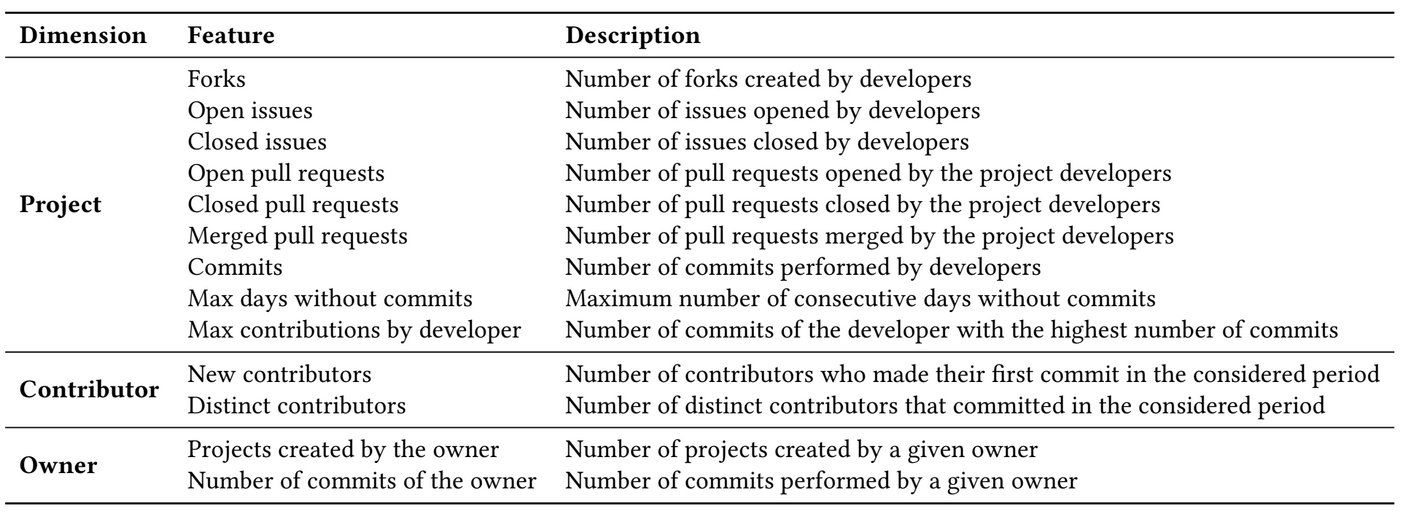
\includegraphics[scale=0.3]{chapters/chapter1/p7-features.png}
    \caption{Features \cite{p:7}}
    \label{fig:p7-features}
\end{figure}

\subsubsection{Models}

Out of ten tested models, Random Forest achieved the best results.
Two baselines were compared: \#1 all projects are predicted as unmaintained and \#2 random predictions.
Models were validated using a 5-fold cross validation.
Six metrics were used to evaluate a performance of classifier:

\begin{enumerate}
    \item precision
    \item recall
    \item F-measure
    \item accuracy
    \item AUC
    \item Kappa
\end{enumerate}

\subsubsection{Results}

The best results -- a precision of 80\% and a recall of 96\% -- were achieved when features were collected for the time period of 2 years in interval of 3 months.
Random Forest also produces a measure of the importance of the features.
The most important features are:

\begin{enumerate}
    \item number of commits
    \item maximal number of days without commits 
    \item maximal contributions by a developer
    \item number of closed issues
\end{enumerate}
